\documentclass[border=0.05cm]{standalone}
\usepackage{../../../../preamble_tikz}

\def\sepArrow{0.56}
\def\sepArrowDouble{0.615}
\def\sepx{0.5}

\begin{document}
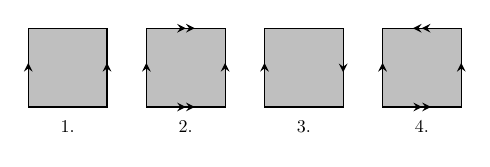
\begin{tikzpicture}
  % SQUARE 1
  \filldraw[fill=lightgray] (0,0) rectangle (1,1);
  % arrows
  \draw [-stealth] (0,0) -- (0,\sepArrow);
  \draw [-stealth] (1,0) -- (1,\sepArrow);
  % label
  \node[anchor=north,scale=0.65] at (0.5,-0.1) {1.};

  % SQUARE 2
  \filldraw[fill=lightgray] (1+\sepx,0) rectangle (2+\sepx,1);
  % arrows
  \draw [-{stealth}{stealth}] (1+\sepx,0) -- (1+\sepx+\sepArrowDouble,0);
  \draw [-stealth] (1+\sepx,0) -- (1+\sepx,\sepArrow);
  \draw [-{stealth}{stealth}] (1+\sepx,1) -- (1+\sepx+\sepArrowDouble,1);
  \draw [-stealth] (2+\sepx,0) -- (2+\sepx,\sepArrow);
  % label
  \node[anchor=north,scale=0.65] at (1+\sepx+0.5,-0.1) {2.};

  % SQUARE 3
  \filldraw[fill=lightgray] (2+2*\sepx,0) rectangle (3+2*\sepx,1);
  % arrows
  \draw [-stealth] (2+2*\sepx,0) -- (2+2*\sepx,\sepArrow);
  \draw [-stealth] (3+2*\sepx,1) -- (3+2*\sepx,1-\sepArrow);
  % label
  \node[anchor=north,scale=0.65] at (2+2*\sepx+0.5,-0.1) {3.};

  % SQUARE 4
  \filldraw[fill=lightgray] (3+3*\sepx,0) rectangle (4+3*\sepx,1);
  % arrows
  \draw [-{stealth}{stealth}] (3+3*\sepx,0) -- (3+3*\sepx+\sepArrowDouble,0);
  \draw [-stealth] (3+3*\sepx,0) -- (3+3*\sepx,\sepArrow);
  \draw [-{stealth}{stealth}] (4+3*\sepx,1) -- (4+3*\sepx-\sepArrowDouble,1);
  \draw [-stealth] (4+3*\sepx,0) -- (4+3*\sepx,\sepArrow);
  % label
  \node[anchor=north,scale=0.65] at (3+3*\sepx+0.5,-0.1) {4.};
\end{tikzpicture}
\end{document}